%%%%%%%%%%%%%%%%%%%%%%%%%%%%%%%%%%%%%%%%%%%%
% https://github.com/martinhelso/uioposter %
%%%%%%%%%%%%%%%%%%%%%%%%%%%%%%%%%%%%%%%%%%%%
% Class options                            %
%%%%%%%%%%%%%%%%%%%%%%%%%%%%%%%%%%%%%%%%%%%%
% Orientation:                             %
% portrait (default), landscape            %
%                                          %
% Paper size:                              %
% a0paper (default), a1paper, a2paper,     %
% a3paper, a4paper, a5paper, a6paper       %
%                                          %
% Language:                                %
% english (default), norsk                 %
%%%%%%%%%%%%%%%%%%%%%%%%%%%%%%%%%%%%%%%%%%%%
\documentclass{uioposter}


\usepackage{lipsum}                                % Dummy text
\usepackage[figwidth = 0.98\linewidth]{todonotes}  % Dummy image (and more!)
\usepackage[absolute, overlay]{textpos}            % Figure placement
\setlength{\TPHorizModule}{\paperwidth}
\setlength{\TPVertModule}{\paperheight}


\title{Uncertainty Estimation with Class Specialized Teacher Ensembles}
\author
{%
    Ryan Marinelli\inst{1}
}
%% Optional:
\institute
{
    \inst{1} Department of Mathematics, University of Oslo
}
% Or:
%\institute{Contact information}


%% Remove footline:
%\setbeamertemplate{footline}{}


\begin{document}
\begin{frame}
\begin{columns}[onlytextwidth]


\begin{column}{0.5\textwidth - 1.5cm}
    \begin{block}{Introduction}
    The medical domain is particularly risk sensitive and requires greater certainty in how AI systems make determinations. Conventional classification approaches often rely on naïve performance metrics, placing emphasis solely on accuracy and overlooking the importance of calibrated confidence in predictions. To address this gap, we investigate an alternative approach: ensembles of specialized models, where each teacher focuses on a subset of the classification task. This study evaluates whether knowledge distillation from such ensembles can improve both predictive certainty and generalization in a multi-class setting.
    \end{block}

    \begin{block}{Motivation}
\textbf{Outer context}: Computer vision models often have a difficult time telling apart items that are closely related and conflate them. This is important in the medical domain which requires greater precision.

\textbf{Research Question:} if you have teachers that specialize in a particular class of image, could a student distill and learn more with multiple teachers?

\textbf{Key motivation}: if combinations of teachers are more effective at transmitting information to a student, wider architecture using Mixture of Experts might be advisable.

\textbf{Prior attempts at Addressing:} Prior work on uncertainty estimation have explored calibration temperature scaling and beta calibration [1,2], as well as stochastic approaches like Monte Carlo dropout [3]. 

\textbf{Why are prior attempts not enough}: Calibration methods often yield global corrections but fail to capture class-specific miscalibration. Monte Carlo dropout reduces certainty but typically underestimates predictive variance. Deep ensembles improve robustness but are computationally expensive and do not explicitly model specialization across classes. 


    \end{block}
\end{column}


\begin{column}{0.5\textwidth - 1.5cm}
    \begin{block}{Methodology}
        A three-class image dataset is used as the testbed(BUSI). We implemented a family of ResNet architectures from the timm library as teacher models, each specialized in learning a single class. Two ensemble setups were compared: (i) a single larger ResNet teacher, and (ii) an ensemble of class-specialized teachers. A smaller student model was trained using knowledge distillation, combining a cross-entropy term on true labels with a KL divergence term aligning the student’s and teacher’s softened outputs. 
    \end{block}

        \begin{block}{Results}
        Using a single teacher to distill the class reaches an accuracy of 81\% with an ECE of .09. Using multiple teachers reaches an accuracy of 76\% with an ECE of .13. Observe Figure 1, the single teacher architecture is more effectively able to teach information through distillation
        
        \begin{figure}
            \centering
            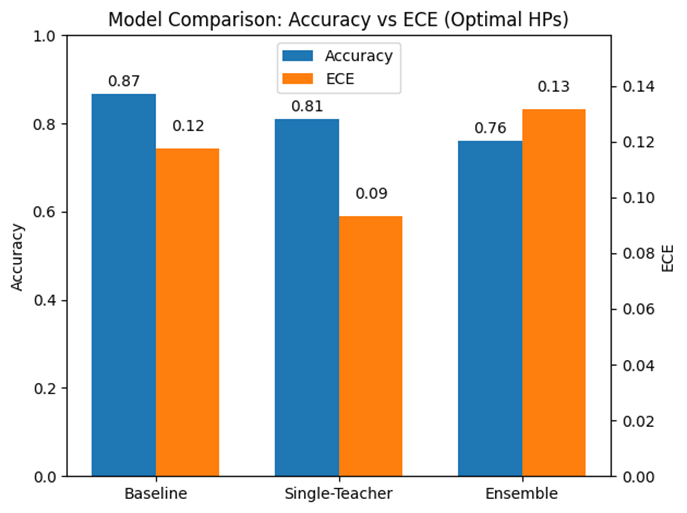
\includegraphics[width=0.5\linewidth]{plot.png}
            \caption{Ensemble Comparison}
            \label{fig:placeholder}
        \end{figure}
        \end{block}


    \begin{block}{Acknowledgments}
       I wanted to thank Dr.Markus Lammle from Upstate University for continued mentorship throughout the project. 

       
    \end{block}

    \begin{block}{References}
\small{
1. Guo, C., Pleiss, G., Sun, Y., & Weinberger, K. Q. (2017). On calibration of modern neural networks. \\
2. Kull, M., Silva Filho, T. M., & Flach, P. (2017). Beyond sigmoids: How to obtain well-calibrated probabilities from binary classifiers with beta calibration. \\
3. Gal, Y., & Ghahramani, Z. (2016). Dropout as a Bayesian approximation: Representing model uncertainty in deep learning. }

    \end{block}

    \begin{block}{Contact information}
    Ryan Marinelli  \\
    Department of Informatics \\
    ryanma@ifi.uio.no
    \end{block}
\end{column}


\end{columns}


\begin{textblock}{0.5}(0.15, 0.92)
    \color{white}
    \sffamily
    \textbf{Department of Informatics}
    \\
    Gaustadalléen 23B, 0373 Oslo, Norway
\end{textblock}


\end{frame}
\end{document}